\documentclass[tikz,border=8pt]{standalone}
\usepackage{amsmath,amssymb}
\usetikzlibrary{arrows.meta,calc,decorations.markings,decorations.pathmorphing,patterns,shapes.geometric,positioning}

\begin{document}
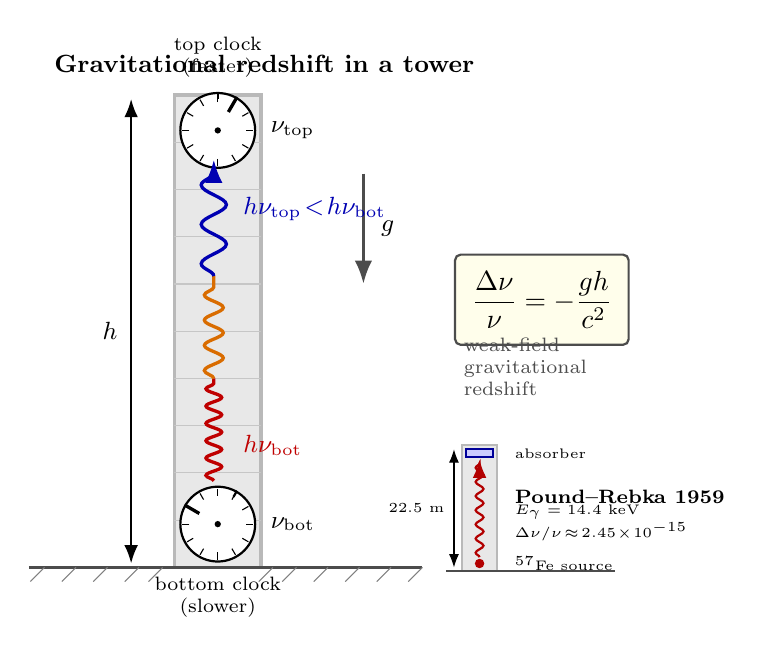
\begin{tikzpicture}[>=Latex,
  clockface/.style={circle, draw=black, thick, fill=white, minimum size=0.95cm, inner sep=0pt},
  formulabox/.style={rectangle, draw=black!70, thick, rounded corners=2pt, fill=yellow!8, inner sep=6pt}]

  % --- Tower outline (gray) -------------------------------------------------
  \fill[gray!18]   (-0.55, 0) rectangle (0.55, 6.0);
  \draw[gray!55, very thick] (-0.55, 0) rectangle (0.55, 6.0);

  % Brick-like horizontal lines on tower
  \foreach \y in {0.6, 1.2, 1.8, 2.4, 3.0, 3.6, 4.2, 4.8, 5.4} {
    \draw[gray!45, thin] (-0.55, \y) -- (0.55, \y);
  }

  % Ground line
  \draw[black!70, thick] (-2.4, 0) -- (2.6, 0);
  \foreach \x in {-2.2, -1.8, -1.4, -1.0, -0.7, 0.7, 1.0, 1.4, 1.8, 2.2, 2.6} {
    \draw[black!50, thin] (\x, 0) -- ($(\x, 0) + (-0.18, -0.18)$);
  }

  % Tower height label h
  \draw[<->, thick] (-1.1, 0.05) -- (-1.1, 5.95);
  \node[font=\small, anchor=east] at (-1.15, 3.0) {$h$};

  % Gravity arrow g
  \draw[->, very thick, black!70] (1.85, 5.0) -- (1.85, 3.6);
  \node[font=\small, anchor=west] at (1.95, 4.3) {$g$};

  % --- Top clock (faster) ---------------------------------------------------
  \node[clockface] (Ctop) at (0, 5.55) {};
  % Hour ticks
  \foreach \a in {0, 30, ..., 330} {
    \draw[black, thin] ($(Ctop) + (\a:0.36)$) -- ($(Ctop) + (\a:0.45)$);
  }
  % Hands: hour pointing ~2 o'clock, minute pointing ~12 (faster: ahead)
  \draw[black, very thick] (Ctop) -- ($(Ctop) + (60:0.27)$);
  \draw[black, thick]      (Ctop) -- ($(Ctop) + (90:0.40)$);
  \fill[black] (Ctop) circle (0.04);
  \node[font=\scriptsize, anchor=south, align=center] at ($(Ctop) + (0, 0.55)$)
    {top clock\\(faster)};
  \node[font=\small, anchor=west] at ($(Ctop) + (0.55, 0)$) {$\nu_{\rm top}$};

  % --- Bottom clock (slower) -----------------------------------------------
  \node[clockface] (Cbot) at (0, 0.55) {};
  \foreach \a in {0, 30, ..., 330} {
    \draw[black, thin] ($(Cbot) + (\a:0.36)$) -- ($(Cbot) + (\a:0.45)$);
  }
  % Hands: hour pointing ~10 o'clock, minute earlier (slower: behind)
  \draw[black, very thick] (Cbot) -- ($(Cbot) + (150:0.27)$);
  \draw[black, thick]      (Cbot) -- ($(Cbot) + (60:0.40)$);
  \fill[black] (Cbot) circle (0.04);
  \node[font=\scriptsize, anchor=north, align=center] at ($(Cbot) + (0, -0.55)$)
    {bottom clock\\(slower)};
  \node[font=\small, anchor=west] at ($(Cbot) + (0.55, 0)$) {$\nu_{\rm bot}$};

  % --- Light wave from bottom to top ---------------------------------------
  % Lower part: short wavelength, red (high frequency)
  \draw[red!75!black, very thick,
        decorate, decoration={snake, amplitude=0.10cm, segment length=0.22cm}]
    (-0.05, 1.10) -- (-0.05, 2.40);
  % Middle part: medium wavelength, orange
  \draw[orange!85!black, very thick,
        decorate, decoration={snake, amplitude=0.12cm, segment length=0.32cm}]
    (-0.05, 2.40) -- (-0.05, 3.70);
  % Upper part: long wavelength, blue (red-shifted: lower frequency)
  \draw[blue!70!black, very thick,
        decorate, decoration={snake, amplitude=0.16cm, segment length=0.50cm}]
    (-0.05, 3.70) -- (-0.05, 5.05);
  % Arrow head at top of wave
  \draw[->, very thick, blue!70!black] (-0.05, 5.05) -- (-0.05, 5.18);

  % Energy labels along the wave
  \node[font=\small, red!75!black, anchor=west] at (0.20, 1.55)
    {$h\nu_{\rm bot}$};
  \node[font=\small, blue!70!black, anchor=west] at (0.20, 4.55)
    {$h\nu_{\rm top}\!<\!h\nu_{\rm bot}$};

  % --- Formula box (right) -------------------------------------------------
  \node[formulabox, anchor=west, align=left] at (3.0, 3.4)
    {$\dfrac{\Delta\nu}{\nu} = -\dfrac{gh}{c^2}$};

  \node[font=\scriptsize, anchor=west, align=left, text=black!70]
    at (3.0, 2.55) {weak-field\\gravitational\\redshift};

  % --- Pound-Rebka inset (lower right) -------------------------------------
  \begin{scope}[shift={(3.1, -0.05)}]
    % Mini tower
    \fill[gray!18] (0.0, 0.0) rectangle (0.45, 1.6);
    \draw[gray!55, thick] (0.0, 0.0) rectangle (0.45, 1.6);
    \draw[black!70, thick] (-0.2, 0.0) -- (1.95, 0.0);

    % Source at bottom
    \fill[red!70!black] (0.225, 0.10) circle (0.06);
    \node[font=\tiny, anchor=west] at (0.55, 0.10) {$^{57}$Fe source};

    % Detector at top
    \draw[fill=blue!20!white, draw=blue!60!black, thick]
      (0.05, 1.45) rectangle (0.40, 1.55);
    \node[font=\tiny, anchor=west] at (0.55, 1.50) {absorber};

    % Photon arrow
    \draw[->, thick, red!70!black,
          decorate, decoration={snake, amplitude=0.05cm, segment length=0.18cm}]
      (0.225, 0.18) -- (0.225, 1.42);

    % Height label
    \draw[<->, thin] (-0.10, 0.05) -- (-0.10, 1.55);
    \node[font=\tiny, anchor=east] at (-0.10, 0.80) {22.5 m};

    % Caption
    \node[font=\scriptsize\bfseries, anchor=west] at (0.55, 0.95)
      {Pound--Rebka 1959};
    \node[font=\tiny, anchor=west, align=left] at (0.55, 0.62)
      {$E_\gamma=14.4$ keV\\$\Delta\nu/\nu\!\approx\!2.45\!\times\!10^{-15}$};
  \end{scope}

  % --- Title arrow / legend ------------------------------------------------
  \node[font=\small\bfseries, anchor=west] at (-2.2, 6.4)
    {Gravitational redshift in a tower};

\end{tikzpicture}
\end{document}
